

\actTitle{Worksheet 4.1-4.4 Review}

\noindent \textbf{Instructions:}  Work together in groups of  3 or 4 to complete the following problems.\\


\begin{enumerate}

\item Consider the angle $\displaystyle \theta=\frac{7\pi}{4}$.
\begin{enumerate}
\item  Draw a picture labeling $\displaystyle \theta=\frac{7\pi}{4}$ and it's corresponding reference angle.\\
\begin{tikzpicture}

\draw[->,ultra thick] (-5,0)--(5,0) node[right]{$x$};
\draw[->,ultra thick] (0,-5)--(0,5) node[above]{$y$};

\end{tikzpicture}

\item Determine the reference angle.
\vfill
\item Determine $\displaystyle \tan\Big(\frac{7\pi}{4}\Big)$.
\end{enumerate}
\vfill

\newpage

%\item Determine the angles, $\theta$, that match the criteria in each question below.
%\begin{enumerate}
%\item An angle that is coterminal with the angle $\alpha=\frac{\pi}{4}$ and is greater than $\pi$.\vfill
%\item An angle that is coterminal with the angle $\alpha=\frac{3\pi}{4}$ and is negative.\vfill
%\end{enumerate}

%\item An angle $\theta$ is in the second quadrant, and $\sin{\theta}=0.25$.  Determine the cosine of the angle.\vfill

\item An angle $\theta$ is in the fourth quadrant, and $\cos{\theta}=0.25$.  Determine the tangent of the angle.\vfill

\item Determine all the angles, $\theta$ between 0 and $3\pi$ such that $\cos{(\theta)}=-\frac{\sqrt{3}}{2}$.  Give exact answers in radians.\vfill




\item The terminal side of an angle $\theta$ in standard position goes through the point $(-6,-5).$  Find an exact answer for the following.
\begin{enumerate}
\item $\sin{(\theta)}$\vfill
\item $\cos{(\theta)}$\vfill
\item $\cot{(\theta)}$\vfill

\end{enumerate}

\newpage

\item For each question below, a diagram of a point on a circle is given.  Answer each question about the angle formed by the line through the point, the origin, and the positive $x$-axis.
\begin{enumerate}
\item Determine the cosine of the angle $\theta$.  (Your answer should be a number and not have an $x$ in it.)\\
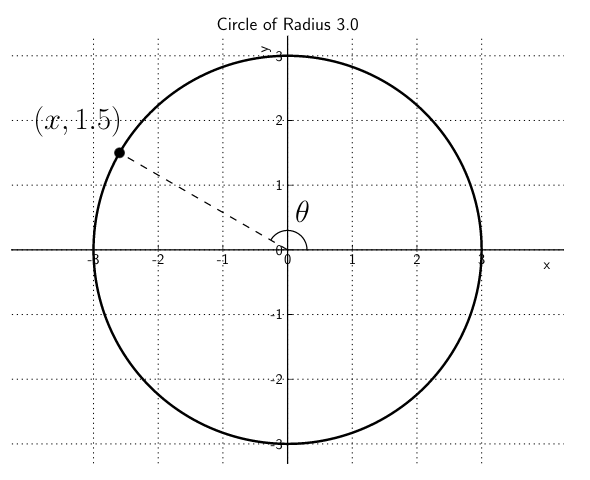
\includegraphics[scale=.7]{circle1}
\item Determine the tangent of the angle $\theta$.  (Your answer should be a number and not have an $x$ in it.)\\
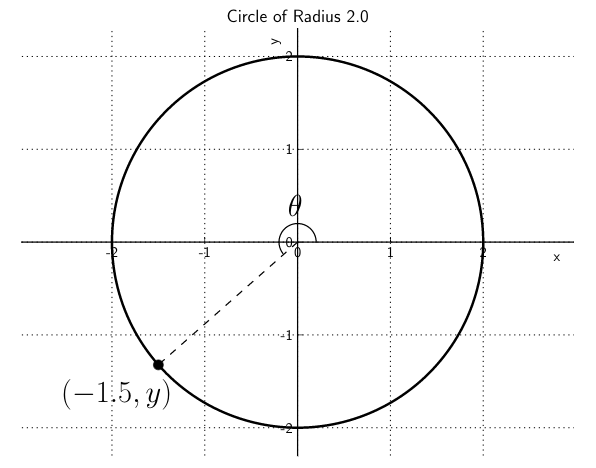
\includegraphics[scale=.7]{circle2}\\

\end{enumerate}






\item Given the following, find the exact value of $\sin{(\theta)}.$\\
$$\cos{(\theta)}=-\frac{1}{3} \quad \text{and}\quad \tan{(\theta)} \quad \text{is negative}$$\vfill

\newpage
\item A ship is anchored a distance of $d=150$ from a beach.  A spotlight on the bow of the ship can rotate, and the angle is measured from a line perpendicular to the beach that goes through the base of the spotlight.  Determine the position, $y$, along the beach that the spotlight will illuminate the given angle, $\theta$.  (Your answer should be a function of $\theta$ with $-\pi/2<\theta <\pi/2.)$\\
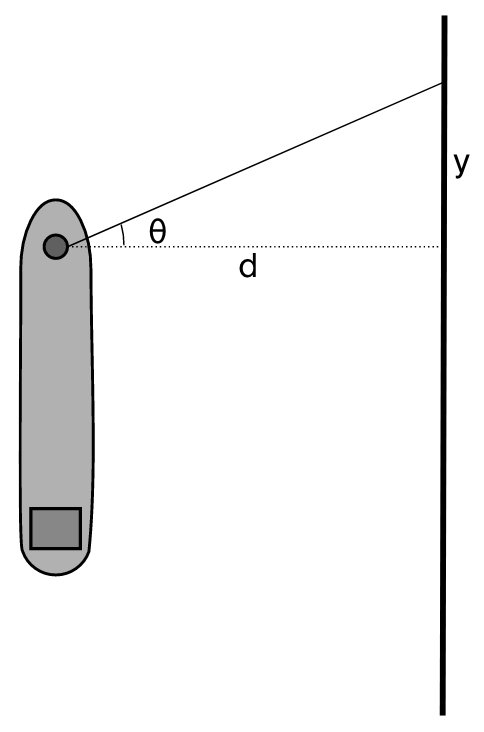
\includegraphics[scale=.4]{ship1}\\

\item Two observers are standing a distance of 100m apart.  They both spot an eagle and watch it closely.  The moment it passes between them, the first observer measures an angle of elevation from the ground of $45^\circ$, and the second observer measures an angle of elevation from the ground of $35^\circ.$  How high in the air was the eagle when it passed between the two observers?\vfill
\vfill




\item A frog rides a unicycle that has a wheel with a diameter of 1.5 inches.  If the frog travels a distance of 320 inches, what is the angle that the wheel turned?  Give an exact answer.\vfill


\newpage


\item A pizza shop owner feels inspired after taking a precalculus class at his local college.  He decides that he wants to sell his 16 inch (diameter) pizzas at a price of \$0.09 per square inch.
\begin{enumerate}
\item Find the price of a slice of pizza as a function of $\theta$.
$$\text{Price}=\text{Area}\times \text{(Price Per Square Inch)}$$\vfill
\item He decides that one slices of pizza must cost \$2.  Find the angle formed by one slice of pizza.  Give your answer \textbf{rounded to the nearest degree}.\vfill
\item About how many slices can he get out of each pizza?\vfill

\end{enumerate}




\item From a point 15 meters above ground level, a surveyor measures the angle of depression of an object on the ground at $68^\circ$.  Approximate the distance from the object to the point on the ground directly beneath the surveyor. (Round to the nearest hundredth.) \vfill
\newpage

\item A surveyor standing 57 meters from the base of a building measures the angle to the top of the building and finds it to be $36^\circ$.  The surveyor then measures the angle to the top of the radio tower on the building and finds it is $50^\circ$.  How tall is the radio tower.  (round to the nearest hundredth).\vfill

\item Find the radian and degree measures of the central angle $\theta$ subtended by the arc of length $s=11$ cm on a circle of radius $r=5$ cm.  Then find the area of the sector determined by $\theta.$  Give an exact answer.\vfill

\item Find the length of the arc $s$ shown in the figure below.  Give an exact answer.\vfil
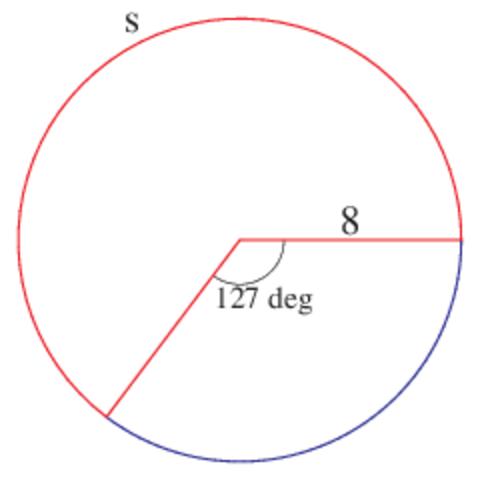
\includegraphics[scale=.5]{redarc}



\end{enumerate}

